%%%%%%%%%%%%%%%%%%%%%%%%%%%%%%%%%%%%%%%%%%%%%%%%%%%
%% LaTeX book template                           %%
%% Author:  Amber Jain (http://amberj.devio.us/) %%
%% License: ISC license                          %%
%%%%%%%%%%%%%%%%%%%%%%%%%%%%%%%%%%%%%%%%%%%%%%%%%%%

\documentclass[a4paper,11pt]{book}
\usepackage[T1]{fontenc}
\usepackage[utf8]{inputenc}
\usepackage{lmodern}
\usepackage{hyperref}
\usepackage{graphicx}
\usepackage[english]{babel}

% title and subtitle
\title{\Huge \textbf{Unified Heteregeneous Networking Middleware Project Report}  \\ 
\huge \vspace{5mm} Fall 2015 }
% Author
\author{\textsc{Jincheng Li}}
\hypersetup{
  urlcolor=blue
}

\begin{document}

\frontmatter
\maketitle

% Auto-generated table of contents, list of figures and list of tables %
\tableofcontents
\mainmatter

% NEW CHAPTER! %
\chapter{Introduction}
Devices with Internet access today are becoming increasingly mobile. The Heterogeneous Networking Middleware project provides a mechanism for devices to seamlessly handle network mobility, and make intelligent decisions about how and when to use different networks across multiple interfaces. \\
The project started in 2012 in the IRT lab and underwent significant development from 2012 to 2013. After a period of inactivity, it was restarted in Spring 2015 and continued until now (Fall 2015). \\
The prototype for this project started with a demo on Linux and is currently shifting to Android. Some work was done last semester to port the Linux implementation to Android, while this semester we took a different approach and re-implemented some of the necessary functionalities within the Android Java Frameork. \\
In this report, I will cover existing work before I started contributing to the project, research on Android framework's networking stack, and what was done this semester to implement the middleware in Android.

\chapter{Existing Work}
Prior to me being involved in the project, a lot of work has been done on the research on heterogeneous networks and Linux prototype implementation. Porting to Android started in Spring 2015. Here we describe the various network protocols used in the project, and the architecture of the Linux prototype.

\section{Protocols}
There are three major protocols involved in the construction of the middleware: HIP, MIP, and MIH. HIP and MIP are two mobility protocols that achieve the same goal: ensuring continuous TCP connection in the presence of IP mobility. MIH is part of the IEEE 802.21 standard, providing an informational service that enables seamless handovers between heterogeneous layer-2 network technologies.

\subsection{HIP}
The Host Identity Protocol

\subsection{MIP}
The Mobile IP protocol

\subsection{MIH}
The Media-Independent Handover protocol

\section{Linux Prototype Architecture}

\chapter{Android Networking Stack}
In order to understand how Android performs network switching and the functionalities it provides similar to MIH, a fair amount of time was spent this semester researching the architecture of Android's networking stack. Here we present the details of our findings.

\section{Android Architecture}
Before we talk about the Android networking stack, we first introduce the architecture of the Android platform. Broadly speaking, Android consists of five layers: Linux kernel, HAL, Android runtime + native libraries, Android Framework, and user applications. These five layers are laid out in the following diagram: % elaborate...

% android architecture diagram here
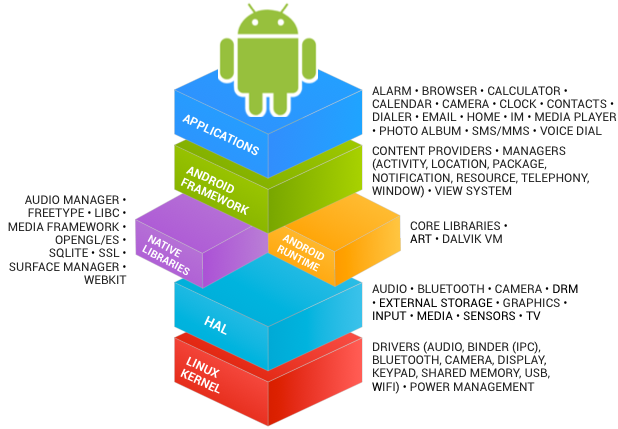
\includegraphics[width=\textwidth]{figures/android_framework_details.png}

At the bottom of the Android software stack is the Linux kernel, which provides a level of abstraction between the device hardware and the upper layers of Android. The kernel provides typical low-level system services such as process, memory management, and also includes essential device drivers for hardware such as cellular and WiFi NICs. \\
The hardware abstraction layer (HAL) defines a standard interface for hardware vendors to implement and allows Android to be agnostic about lower-level driver implementations. We don't discuss HAL at any more length here as it is not vital for our purposes. \\
Next comes the Android runtime (i.e. Davlik VM) and native libraries, which are implemented in C/C++. \\
Layered on top of the runtime and libraries is the Android Framework. This framework is implemented entirely in Java, and provides applications with an API that can be used to interact with system services, including UI, telephony, location, etc. This part of Android is what most of the research effort on Android this semester focused on. The final demo also directly modifies Android Framework's source code to integrate our middleware functionalities into the system. \\
Finally on the top level is user applications that interact directly with the user. 

\section{General Networking}
The following classes deal with network connectivity for all types of networks (cellular, WiFi, or ethernet). This is done through an abstraction called NetworkAgent that encapsulates different types of networks into a common interface, as is explained in more detail later in this section.

\subsection{ConnectivityManager}
In general, classes with a ``Manager'' suffix are singleton classes exposed as part of the Android API for applications. They serve as the interface between application developers and the Android framework. Methods in these classes do not usually contain intricate program logic, but simply call some other system service class (e.g. methods in ConnectivityManager call corresponding methods in ConnectivtyService) which actually implements the required functionality. \\
In the case of ConnectivityManager, it is reponsible for answering queries about the state of network connectivity, and for notifying applications about network connectivity changes. Additionally, it allows applications to request or select certain networks for their data traffic. This last feature is most relevant to our research, as it provides an entry point for applications to specify the characteristics of the network they prefer. It is essentially a simplified version of the middleware's policy engine. An application can choose a policy for its network traffic, and Android will match the network that scores the highest according to that policy to this application. \\
The method invoked for applications to request certain networks is \verb|requestNetwork|, which takes as its input a \verb|NetworkRequest|, and a \verb|NetworkCallback|. As its name suggests, the \verb|NetworkCallback| is invoked once the network is switched to one that satisfies the request. The key component of a \verb|NetworkRequest| is a \verb|NetworkCapabilities| object, representing the capabilities of a network. 


\subsection{ConnectivityService}
\verb|ConnectivityService| provides implementations of many methods in \verb|ConnectivityManager|.

\subsection{NetworkAgent and NetworkAgentInfo}

\section{WiFi Networks}

\subsection{WifiManager}
The WifiManager class is exposed as part of Android's application API. It provides methods for applications to manage all aspects of WiFi connectivity.

\subsection{WifiService}

\subsection{WifiStateMachine}

\subsection{WifiAutoJoinController}

\section{Cellular Networks}
\subsection{TelephonyManager}
\subsection{DataConnection}

\section{Another section heading}
Lorem ipsum dolor sit amet, consectetur adipisicing elit, sed do eiusmod tempor incididunt ut labore et dolore magna aliqua. Ut enim ad minim veniam, quis nostrud exercitation ullamco laboris nisi ut aliquip ex ea commodo consequat.

% Sample table                                        %
% Source: www1.maths.leeds.ac.uk/latex/TableHelp1.pdf %
\begin{table}[ht]
\caption{Sample table} % title of Table
\centering % used for centering table
\begin{tabular}{c c c c}
% centered columns (4 columns)
\hline\hline %inserts double horizontal lines
S. No. & Column\#1 & Column\#2 & Column\#3 \\ [0.5ex]
% inserts table
% heading
\hline % inserts single horizontal line
1 & 50 & 837 & 970 \\
2 & 47 & 877 & 230 \\
3 & 31 & 25 & 415 \\
4 & 35 & 144 & 2356 \\
5 & 45 & 300 & 556 \\ [1ex] % [1ex] adds vertical space
\hline %inserts single line
\end{tabular}
\label{table:nonlin} % is used to refer this table in the text
\end{table}

\chapter{Implementation in Android}

\section{Working with the Android Framework}
This section describes the necessary steps to set up and work with the Android framework. Most of this information can also be found on the Android Open-Source Project (AOSP: \url{https://source.android.com/source}) site. This guide simply documents the specific steps I went through in this project. \\

\subsection{Environment Setup}

\subsubsection{Requirements}
Developing AOSP typically requires a 64-bit Linux or Mac OS system. I'm using 64-bit Linux Mint 17. As such, the following documentation applies to Linux only (note that Ubuntu should behave the same way as Linux Mint). For more reference on Mac OS, please refer to the AOSP site. Also note that 150 GB of free disk space is recommended for a single build.

\subsubsection{Establishing Build Environment}
Please see the page on AOSP (\url{https://source.android.com/source/initializing.html}) for reference on properly setting up dependencies for the build environment. These are simply some \verb|apt-get| commands and configurations. Note that at the end of the page there is a section called ``Optimizing a build environment'', which enables ccache to speed up recompilation. In my experience this was very helpful for saving compilation time. \\

\subsubsection{Downloading Android Source}
To download the Android source, you first need to have the \verb|repo| tool installed. This can be done with:
\begin{verbatim}
$ sudo curl https://storage.googleapis.com/git-repo-downloads/repo 
  > /usr/local/bin/repo
$ sudo chmod a+x /usr/local/bin/repo
\end{verbatim}
Next, create an empty directory to hold your working files:
\begin{verbatim}
$ mkdir ~/android
\end{verbatim}
Run \verb|repo init| to bring down the latest version of the \verb|repo| tool, and also supply it with a URL for the manifest, which specifies where the various repositories included in the Android source will be placed within your working directory.
\begin{verbatim}
$ repo init -u 
  https://android.googlesource.com/platform/manifest
\end{verbatim}
Note that this defaults to the \verb|master| branch, which is the one I developed on. At the time of writing, the Android version for the \verb|master| branch is 6.0 Marshmallow. It is also possible to download a different version of Android using a different manifest file. \\
Once the initialization is complete, run
\begin{verbatim}
$ repo sync
\end{verbatim}
to pull down the Android source tree. This should take anywhere between an hour to ten hours depending on your connection bandwidth. It is okay to interrupt the process. Running \verb|repo sync| again later will pick up from where the download was left off.

\subsection{Building and Running}
There are two ways to build/run the source code: with an emulator, or with a physical device. The emulator is a bit slow and lacks support for WiFi networks. It runs inside a QEMU hypervisor and has an emulated cellular connection. For physical devices, the only devices that AOSP currently supports are Nexus devices. Any other device requires a build configuration that's not directly available in the provided \verb|lunch| menu. You can find some useful information about non-Nexus device configurations on the CyanogenMod wiki (\url{https://wiki.cyanogenmod.org/w/Main_Page}).
\subsubsection{Building}
First, initialize the build environment by sourcing the \verb|envsetup.sh| script. Inside \verb|~/android| (where Android source is downloaded to), run
\begin{verbatim}
$ source build/envsetup.sh
\end{verbatim}
This includes several utility functions into the shell, which are necessary for building the source. Note that only \verb|bash| is compatible with these functions, so make sure you are not using another shell. \\
Next, choose a target to build with \verb|lunch|. You can see a list of possible targets by running \verb|lunch| without an argument, or you can choose a target directly with, for instance,
\begin{verbatim}
$ lunch aosp-arm_eng
\end{verbatim}
which builds the emulator with all debugging enabled. \\
Finally, build everything with \verb|make|. It is recommended to build using the \verb|-jN| argument, which parallelizes the build process. The fastest builds are ususally made with number of tasks N between 1 and 2 times the number of hardware threads on the computer. For example, for a computer with 8 cores, the fastest builds are between \verb|make -j8| and \verb|make -j16|.
\subsubsection{Running}
To run an emulator build, simply run \verb|emulator| in the terminal. To run a device-specific build, you can flash it onto the device with \verb|fastboot|. In order to flash a device, connect the device to your computer, and run
\begin{verbatim}
$ adb reboot bootloader
\end{verbatim}
which reboots the device into fastboot mode, and then run
\begin{verbatim}
$ fastboot flashall -w
\end{verbatim}
which flashes the system image onto the device.\\
For more information on running builds and choosing the appropriate build configuration for a device, see \url{https://source.android.com/source/running.html}.

\subsection{Developing}
As previously mentioned, \verb|repo| is used to manage development of the Android project. Development of a new topic branch typically starts with
\begin{verbatim}
$ repo start <BRANCH_NAME> [<PROJECT_LIST>]
\end{verbatim}
This will create a branch with the given name in each of the \verb|git| projects included in \verb|<PROJECT_LIST>|. Afterwards, simply proceed as usual to each of the projects, make some changes, and commit them separately with \verb|git|. You can use \verb|repo status [<PROJECT_LIST>]| to check the status of each of the projects. \\
Unfortunately there is no easy way to upload your changes to a remote repository. For now I have saved my changes as \verb|diff| files and uploaded them to my GitHub repository, but this is obviously not a great approach. The \verb|repo| tool is designed to let you upload your changes to the Google source code server and submit them for review, eventually merging into the \verb|master| branch. However, since we are working on an experimental project with limited time, this is not a desired method either. \\


\section{Final Demo}

\end{document}
